\section{Leitner's learning box reviewed}

% Mention the visual validation tool?
\emph{Leitner's learning box}\footnote{http://en.wikipedia.org/wiki/Leitner\_system} is a simple, but ingenious little contraption to support the tedious
process of memorization, especially prominent when trying to learn, for example, a new language. As depicted in Fig.~\ref{fig:membox_depiction}, this box
consists of a series of partitions with a strict set of rules. The contents to be memorized are written on little cards and placed in the first container. Every
time the user correctly answers a card, that card is promoted to the next partition. Once it reaches the final partition, it can be considered memorized, and
no longer needs to be practiced. Every time the user incorrectly answers a card however, it is sent back to the original starting partition, and the
learning process is restarted.

\begin{figure}[htbp]
	\centering
  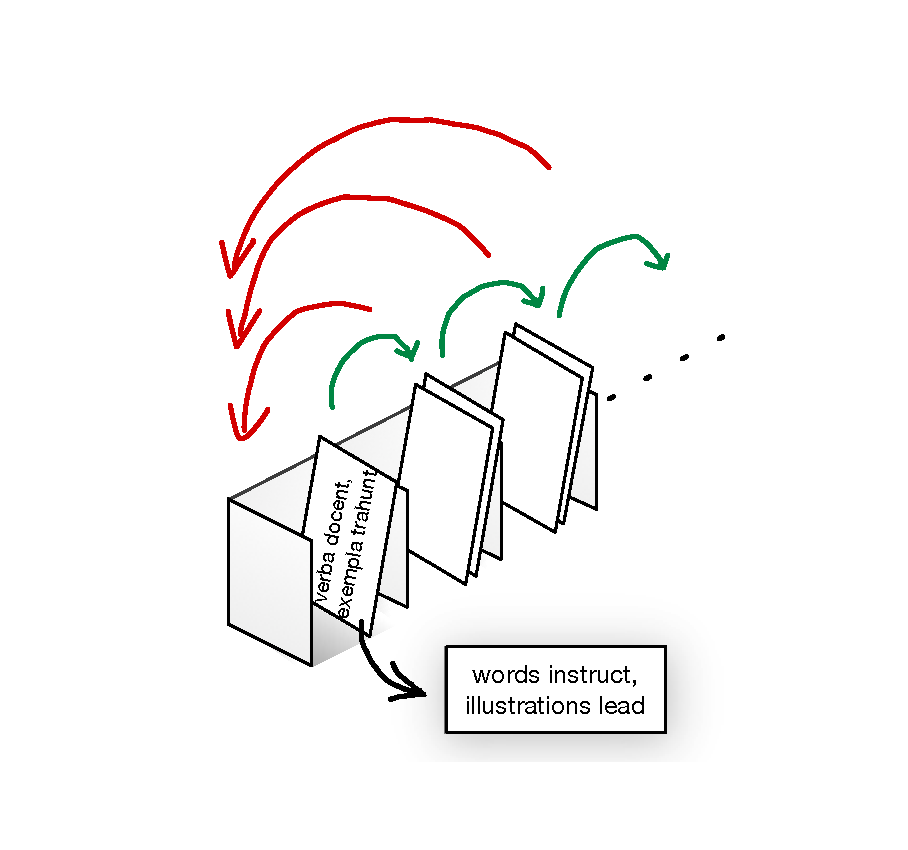
\includegraphics[width=0.4\textwidth]{membox_illustration.pdf}
	\caption{Static Structure of a Leitner's Learning Box}
	\label{fig:membox_depiction}
\end{figure}
\FloatBarrier

For a more detailed overview of the box and our goals, we recommend you read the introduction to Part II. But for now, enough discussion!

\begin{itemize}

\item[$\blacktriangleright$] To get started, press the \texttt{new} button and navigate to ``Examples/eMoflon Handbook Examples/''
(Fig.~\ref{fig:downloadWizard}).

\begin{figure}[htbp]
	\centering
  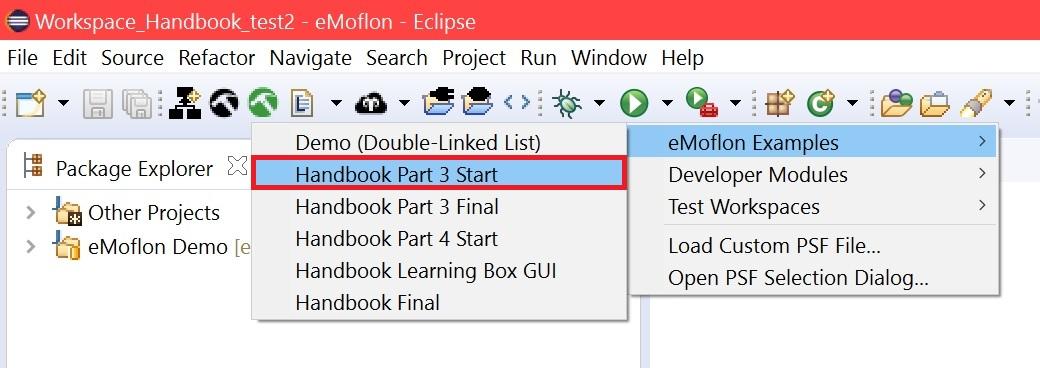
\includegraphics[width=0.75\textwidth]{eclipse_downloadWizard}
	\caption{Download the file set to get started}
	\label{fig:downloadWizard}
\end{figure}
\FloatBarrier

\item[$\blacktriangleright$] Download the file package of the eMolfon syntax type you'd like to learn about. Remember, with the visual syntax, you'll be using
an external modeling program to craft your metamodel diagrams, then exporting the data to Eclipse. With textual, you'll be working entirely within the
Eclipse IDE in the eMolfon perspective.

\item[$\blacktriangleright$] If your package explorer does not resemble ours in Fig.~\ref{fig:workingSets} with at least two distinct nodes, select the
small, downward facing arrow in the corner of the module window. Choose ``Working Sets'' as your ``Top Level Elements''. We work with many working sets, and use
them to structure the workspace in Eclipse.
\end{itemize}

The ``MyWorkingSet" node contains \texttt{LeitnersLearningBox}, which in turns contains all the metamodel project files. Visually, this is represented in a
single \texttt{.eap} file. In the textual syntax, it is a specific project structure with several classes. The model generated from the metamodel can be found
under the second node, in \texttt{LearningBoxLanguage}. These sets are not contained within the same node because they are different \emph{nature}s, or
project types. \texttt{LearningBoxLanguage} is your \emph{repository project}, the Eclipse classification for a normal Java project\footnote{For more details
on the project structure, review section 4 of Part I.}. 

\begin{figure}[htbp]
	\centering
  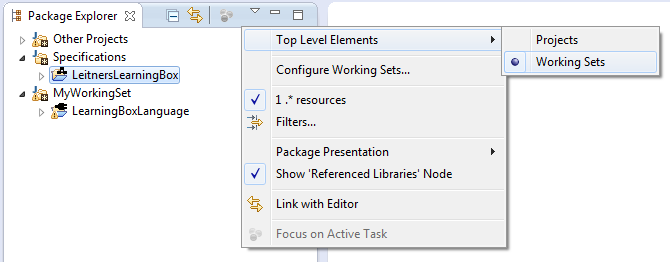
\includegraphics[width=0.9\textwidth]{eclipse_workingSets}
	\caption{Setting your Package Explorer}
	\label{fig:workingSets}
\end{figure}
\FloatBarrier

\begin{itemize}
% THINK: Is this information actually helpful for the user?
\item[$\blacktriangleright$] Inspect the files until you feel comfortable with what you'll be working with. In particular, look at your metamodel structure in
the \texttt{MOSL} folder. Everything defined here is also defined in the \texttt{.ecore} model file in ``LearningBoxLanguage/model/''. You can review how to
create a dynamic instance of your model in section 4 of Part II. We have included a small instance in your download, but encourage experimentation. We also
invite you to browse the files in \texttt{gen}, especially each of the \texttt{.impl} files. You'll find the each implementation file includes an
empty method declaration for each signature declared in the metamodel\footnote{For specific details on their contents, refer to Part II, section 5.}.

\item[$\blacktriangleright$] Well, that's it! A quick review, paired with a fine download makes an excellent appetizer to SDMs. Let's get started.

\end{itemize}
